\begin{pastexam}[label={px:gw3-109-ds-02}]{關務三等資訊處理 109 年 第二題}
（申論；20 分）

給定一個無向圖（Undirected Graph）G 的鄰接列表（Adjacency List）如圖，試依據該列表提供的資訊繪製出對應的無向圖 G，然後由節點（Vertex）H 為起始點繪製 Depth First Search（DFS）與 Breadth First Search（BFS）生成樹（Spanning Tree），遇有多個節點可被走訪時，字母順序越前面的節點，其被走訪的優先順序就越高。（20 分）
\begin{center}
\begin{tikzpicture}[x=1cm,y=0.62cm,>={Stealth[length=1.6mm]},
  h/.style={draw,minimum width=6mm,minimum height=6.2mm,inner sep=0pt,font=\small\sffamily},
  c/.style={draw,minimum width=5.5mm,minimum height=5mm,inner sep=0pt,font=\small\sffamily},
  p/.style={draw,minimum width=5mm,minimum height=5mm,inner sep=0pt}]
\foreach \v/\lst [count=\r] in {A/{B,C}, B/{A,D,E}, C/{A,F,G}, D/{B,H}, E/{B,H}, F/{C,H}, G/{C,H}, H/{D,E,F,G}} {
  \node[h] (h\r) at (0,-\r) {\v};
  \foreach \u [count=\k] in \lst {
    \node[c] (c\r-\k) at (0.75+1.45*\k,-\r) {\u};
    \node[p,anchor=west] (p\r-\k) at (c\r-\k.east) {};
  }
}
\foreach \r/\m in {1/2, 2/3, 3/3, 4/2, 5/2, 6/2, 7/2, 8/4} {
  \draw[->] (h\r.east) -- (c\r-1.west);
  \foreach \k [evaluate=\k as \kk using int(\k+1)] in {1,...,\m} {
    \ifnum\k<\m \draw[->] (p\r-\k.center) -- (c\r-\kk.west); \fi
  }
}
\node at (2.6,-9.2) {無向圖 G 鄰接列表};
\end{tikzpicture}
\end{center}
\end{pastexam}

\begin{pastsoln}
DFS、BFS 與生成樹見資結書第~21.3、21.4~節。 鄰接列表中每條無向邊在兩端各出現一次。 共 $20$ 個串列節點，所以 G 有 $10$ 條邊：A–B、A–C、B–D、B–E、
C–F、C–G、D–H、E–H、F–H、G–H（逐一檢查，例如 B 的串列有 D、D 的串列也有 B，列表是對稱的）。

\textbf{無向圖 G}：
\begin{center}
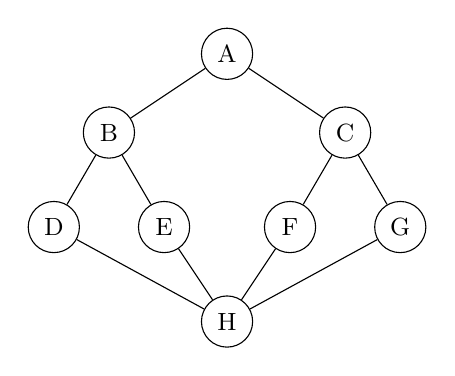
\begin{tikzpicture}[x=1cm,y=1cm,v/.style={circle,draw,minimum size=6.5mm,inner sep=0pt,font=\small}]
\node[v] (A) at (0,2.4) {A};
\node[v] (B) at (-1.5,1.4) {B}; \node[v] (C) at (1.5,1.4) {C};
\node[v] (D) at (-2.2,0.2) {D}; \node[v] (E) at (-0.8,0.2) {E};
\node[v] (F) at (0.8,0.2) {F}; \node[v] (G) at (2.2,0.2) {G};
\node[v] (H) at (0,-1.0) {H};
\foreach \a/\b in {A/B,A/C,B/D,B/E,C/F,C/G,D/H,E/H,F/H,G/H} \draw (\a)--(\b);
\end{tikzpicture}
\end{center}

\textbf{DFS（從 H）}。 每到一個節點，依字母順序找第一個還沒走過的鄰居往下走；都走過了就退回上一個節點。
\begin{center}
\small
\begin{tabular}{lll}
\toprule
目前節點 & 鄰居（字母順序） & 動作 \\
\midrule
H & D, E, F, G & 走到 D（樹邊 H–D） \\
D & B, H & 走到 B（D–B） \\
B & A, D, E & 走到 A（B–A） \\
A & B, C & B 走過，走到 C（A–C） \\
C & A, F, G & A 走過，走到 F（C–F） \\
F & C, H & 都走過，退回 C \\
C & & 走到 G（C–G） \\
G & C, H & 都走過，退回 C、A，回到 B \\
B & & D 走過，走到 E（B–E） \\
E & B, H & 都走過，退回 B、D、H，結束 \\
\bottomrule
\end{tabular}
\end{center}
走訪順序 H, D, B, A, C, F, G, E。 DFS 生成樹的邊：H–D、D–B、B–A、A–C、C–F、C–G、B–E。

\textbf{BFS（從 H）}。 用佇列，取出一個節點，依字母順序把還沒走過的鄰居都標記並放入佇列。
\begin{center}
\small
\begin{tabular}{lll}
\toprule
取出 & 新加入（樹邊） & 佇列 \\
\midrule
（開始） & H & H \\
H & D、E、F、G（H–D、H–E、H–F、H–G） & D, E, F, G \\
D & B（D–B） & E, F, G, B \\
E & （B 已標記） & F, G, B \\
F & C（F–C） & G, B, C \\
G & （C 已標記） & B, C \\
B & A（B–A） & C, A \\
C & （A 已標記） & A \\
A & & 空 \\
\bottomrule
\end{tabular}
\end{center}
走訪順序 H, D, E, F, G, B, C, A。 BFS 生成樹的邊：H–D、H–E、H–F、H–G、D–B、F–C、B–A。

\textbf{兩棵生成樹}（以 H 為根畫）：
\begin{center}
\begin{tikzpicture}[level distance=10mm,every node/.style={circle,draw,minimum size=6.5mm,inner sep=0pt,font=\small},
  level 4/.style={sibling distance=16mm},level 5/.style={sibling distance=12mm}]
\node {H}
  child {node {D}
    child {node {B}
      child {node {A} child {node {C} child {node {F}} child {node {G}}}}
      child {node {E}}}};
\node[draw=none,font=\small] at (0,-6.4) {DFS 生成樹};
\end{tikzpicture}
\qquad\qquad
\begin{tikzpicture}[level distance=10mm,every node/.style={circle,draw,minimum size=6.5mm,inner sep=0pt,font=\small},
  level 1/.style={sibling distance=13mm}]
\node {H}
  child {node {D} child {node {B} child {node {A}}}}
  child {node {E}}
  child {node {F} child {node {C}}}
  child {node {G}};
\node[draw=none,font=\small] at (0,-6.4) {BFS 生成樹};
\end{tikzpicture}
\end{center}
兩棵都有 $8$ 個節點、$7$ 條邊。 DFS 樹又深又窄（深度 $5$），BFS 樹的每個節點都在它離 H 的最短距離那一層（例如 A 離 H 最少 $3$ 條邊，在第 $3$ 層）。
\end{pastsoln}
